\newpage
\section{Conceitos e Tecnologias Utilizadas}

\par Este capítulo aborda os conceitos e as tecnologias que sustentam o trabalho: automação industrial, tecnologia da informação aplicada ao contexto industrial e desenvolvimento de software. O objetivo é reunir as definições, os enquadramentos e as ferramentas necessários para compreender um sistema supervisório web orientado a serviços. Os temas partem da fundamentação do supervisório e da automação, passam pela infraestrutura de execução, pelo armazenamento de dados, pelas tecnologias de aplicação e de segurança e chegam ao protocolo de comunicação com os equipamentos de campo.

\subsection{Sistema SCADA}

\par A indústria evoluiu muito na busca por mais monitoramento e controle dos processos. Com o tempo, os custos de computadores, hubs e conversores de rede caíram bastante, ao passo que o desenvolvimento de software ganhava relevância. \cite{AHMED2011_EFFICIENT_WEB_SCADA} Nesse contexto, as empresas de software industrial passaram a oferecer soluções personalizadas para cada tipo de processo e indústria, com ampla gama de protocolos de comunicação. A esse tipo de sistema deu-se o nome de \sigla{scada}, sigla em inglês para \emph{Supervisory Control and Data Acquisition} \cite{ZANGHI2019_SCADA_CONCEITOS}. De forma geral, define-se o \sigla{scada} como um pacote de software posicionado sobre o hardware ao qual se interliga, que viabiliza a supervisão e o controle de processos industriais de forma local ou remota \cite{PHUYAL2020_COST_EFFICIENT_SCADA}.

\par A aplicação dos sistemas \sigla{scada} estende-se a praticamente todos os segmentos que operam processos distribuídos e de funcionamento contínuo, muitos deles classificados como infraestruturas críticas, cuja interrupção compromete serviços essenciais \cite{YADAV2020_SCADA_ARCHITECTURE_REVIEW}. Entre os usos típicos estão a geração, a transmissão e a distribuição de energia elétrica, o tratamento e a distribuição de água e o saneamento, a produção e o transporte de óleo e gás por dutos, os sistemas de transporte, as indústrias química e farmacêutica, a produção de papel e celulose, o setor de alimentos e bebidas e a manufatura discreta, como a automotiva e a aeroespacial \cite{STOUFFER2015_NIST_ICS_SECURITY}. A Figura~\ref{fig:ihm_scada} ilustra uma tela de supervisão.

\begin{figure}[H]
    \centering
    \caption{Tela de Supervisão}
    \centering
    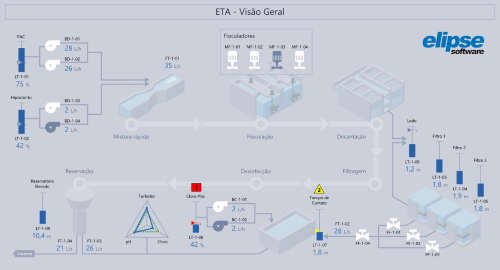
\includegraphics[width=0.85\textwidth]{Imagens/Desenvolvimento/Cap1/scada.png}
    \centering
    \vspace{0.2cm} \\
    Fonte: \textcite{ELIPSE_IHM_ALTA_PERFORMANCE}.
    \label{fig:ihm_scada}
\end{figure}

\par Para \textcite{ZANGHI2019_SCADA_CONCEITOS}, um sistema \sigla{scada} deve contemplar seis módulos, descritos nas subseções a seguir: aquisição e registro de dados, sincronismo de tempo, níveis de acesso, comando e controle, escalabilidade e redundância.

\subsubsection{Aquisição e Registro de Dados}

\par A aquisição das informações de campo é o primeiro grande desafio em um sistema \sigla{scada} \cite{ZANGHI2019_SCADA_CONCEITOS}. Atualmente, predominam dispositivos genéricos inteligentes que disponibilizam algum protocolo de comunicação, responsáveis por adquirir grandezas analógicas e digitais e disponibilizá-las ao supervisório em formato binário por meio de uma rede de dados \cite{YADAV2020_SCADA_ARCHITECTURE_REVIEW}. O meio de comunicação varia conforme a distância e a infraestrutura disponível, indo das redes locais cabeadas, tipicamente Ethernet, a enlaces sem fio como rádio frequência (\sigla{rf}) e telefonia móvel (4G) \cite{STOUFFER2015_NIST_ICS_SECURITY}, até soluções orientadas à Internet das Coisas, que trafegam os dados pela internet \cite{KHALID2024_IOT_SCADA_PHOTOVOLTAIC}.

\par Os pontos adquiridos em um sistema \sigla{scada} são denominados \emph{tags} e armazenados no banco de dados do supervisório. Cada tag assume um tipo de dado conforme a natureza da grandeza que representa, podendo ser booleano, inteiro, real ou texto. O registro contínuo desses valores pelo supervisório permite análises posteriores, na forma de gráficos históricos de tendência e de sequenciais de eventos \cite{ZANGHI2019_SCADA_CONCEITOS}.

\subsubsection{Sincronismo de Tempo}

\par Outro requisito fundamental dos sistemas \sigla{scada} é o sincronismo de tempo. Todo dado coletado deve possuir um registro de tempo de origem, a chamada estampa de tempo (\emph{time stamp}), de modo que cada variação de estado fique associada a um instante de referência. Essa exigência decorre da necessidade de análises posteriores de ocorrências e faltas, que dependem da cronologia precisa dos acontecimentos para permitir a identificação das causas \cite{ZANGHI2019_SCADA_CONCEITOS}.

\par Na prática, a aquisição é realizada de forma cíclica: o supervisório consulta periodicamente os dispositivos de campo, processo conhecido como \emph{polling} \cite{STOUFFER2015_NIST_ICS_SECURITY}, em ciclos de leitura sucessivos cuja frequência é definida conforme a dinâmica do processo \cite{YADAV2020_SCADA_ARCHITECTURE_REVIEW}. Como consequência, a estampa de tempo atribuída a cada ponto corresponde ao ciclo em que o valor foi lido, e não ao instante físico exato da transição, de modo que a resolução temporal do registro fica limitada ao período do ciclo de aquisição.

\subsubsection{Níveis de Acesso}

\par Os níveis de acesso de um sistema \sigla{scada} definem a separação das permissões de supervisão e controle entre os usuários. Classicamente organizada em níveis por instalação \cite{ZANGHI2019_SCADA_CONCEITOS}, essa separação materializa-se como acessos definidos por planta, em que cada usuário recebe permissões apenas sobre os pontos e comandos da instalação à qual está vinculado, segundo o controle de acesso baseado em cargos e o princípio do menor privilégio, apoiado em mecanismos adequados de autenticação e autorização \cite{STOUFFER2015_NIST_ICS_SECURITY}.

\subsubsection{Comando e Controle}

\par As ações executadas remotamente pelo supervisório consistem no envio de comandos aos dispositivos de campo, isto é, na escrita de uma informação no dispositivo \cite{YADAV2020_SCADA_ARCHITECTURE_REVIEW}. Quanto ao momento de execução, o comando pode ser instantâneo, escrevendo de imediato o valor desejado ou agendado, programado para ações conforme cenários previamente definidos, com o instante de execução registrado \cite{ZANGHI2019_SCADA_CONCEITOS}.

\par O processamento de um comando segue quatro fases: seleção, em que o operador escolhe na interface o equipamento; verificação de intertravamentos e condições de segurança; confirmação explícita pelo operador; e execução, com o envio efetivo da ordem ao elemento final de controle \cite{ZANGHI2019_SCADA_CONCEITOS}. Após a execução, o supervisório verifica a confirmação para garantir que a solicitação foi aceita pelo dispositivo e, em caso de falha, gera um alarme, pois comandos indevidos podem danificar equipamentos ou comprometer a segurança do processo \cite{STOUFFER2015_NIST_ICS_SECURITY}.

\subsubsection{Escalabilidade}

\par A expansão das instalações é frequente em ambientes industriais, com a inclusão de novos equipamentos, pontos de medição e circuitos. Para acompanhá-la, o software \sigla{scada} deve ser escalável, permitindo acrescentar pontos à base de dados e criar novas telas de operação sem comprometer o que já está em produção \cite{ZANGHI2019_SCADA_CONCEITOS}.

\par A análise da escalabilidade deve abranger não apenas o supervisório, mas também os elementos de aquisição, controle e rede, que precisam permitir o acréscimo de novos dispositivos ao barramento de comunicação, integração a ser prevista já na fase inicial do projeto \cite{ZANGHI2019_SCADA_CONCEITOS}.

\subsubsection{Redundância}

\par A redundância consiste no acréscimo de um elemento idêntico ao original, de modo que, em caso de falha do primeiro, o segundo assuma suas funções da forma mais transparente possível para a operação \cite{ZANGHI2019_SCADA_CONCEITOS}. A prática aplica-se a diversos componentes do sistema, como softwares supervisórios, dispositivos de aquisição e controle e elementos de rede, apesar do custo adicional, eleva a confiabilidade a graus compatíveis com a criticidade de aplicações industriais sensíveis.

\par Em uma arquitetura redundante típica, múltiplas estações de operação comunicam-se simultaneamente com os dispositivos de campo e as unidades de aquisição e controle operam em pares espelhados \cite{ZANGHI2019_SCADA_CONCEITOS}. De modo geral, recomenda-se que cada componente crítico tenha um par redundante, sobre redes igualmente redundantes, e que o sistema seja projetado para degradação suave, preservando a supervisão e o controle mesmo diante de falhas pontuais \cite{STOUFFER2015_NIST_ICS_SECURITY}.

\subsection{Ajuste para Escala de Engenharia e Linearização de Sensores}

\par Os sensores e transmissores de campo convertem uma grandeza física, como pressão, nível, temperatura ou vazão, em um sinal elétrico padronizado. Os padrões mais difundidos são a corrente de 4 a 20\,mA e a tensão de 0 a 10\,V. A faixa de 4 a 20\,mA é preferida em instalações industriais porque a corrente é menos sensível a ruído e à queda de tensão em cabos longos, e porque o início da faixa em 4\,mA, e não em 0\,mA, permite distinguir uma medição no valor mínimo de uma falha do circuito, como o rompimento do cabo, que leva a corrente a zero.

\par O sinal elétrico, no entanto, não chega ao supervisório como uma grandeza física. Ele é digitalizado por um conversor analógico-digital (A/D), que entrega um número inteiro, o valor bruto, cuja faixa depende da resolução em bits do conversor. Um conversor de 12 bits, por exemplo, representa o fundo de escala com 4096 níveis, de 0 a 4095 contagens. O ajuste para escala de engenharia é a operação que transforma esse valor bruto na grandeza que o operador reconhece, expressa na unidade de engenharia (u.e.) correspondente, como bar, metro ou litro por segundo.

\par Quando a relação entre o sinal e a grandeza é linear, a conversão é uma reta, como mostra a Equação~\ref{eq:cap2_reta}, em que $x$ é o valor bruto, $y$ é o valor em unidade de engenharia, $a$ é o ganho e $b$ é o deslocamento, também chamado de \emph{offset}.

\myequation{y = a \cdot x + b}{eq:cap2_reta}{Conversão linear do valor bruto para a unidade de engenharia}{\text{u.e.}}

\par Os dois coeficientes são determinados por dois pontos de calibração conhecidos, o limite inferior e o limite superior da faixa, em que $x_\text{min}$ e $x_\text{max}$ são os valores brutos nos extremos e $y_\text{min}$ e $y_\text{max}$ são as grandezas correspondentes. Impondo que a reta passe pelos dois pontos, obtém-se o sistema da Equação~\ref{eq:cap2_sistema}, cuja solução fornece o ganho, na Equação~\ref{eq:cap2_ganho}, e o deslocamento, na Equação~\ref{eq:cap2_offset}.

\begin{equation}
    \begin{cases}
        y_\text{min} = a \cdot x_\text{min} + b \\
        y_\text{max} = a \cdot x_\text{max} + b
    \end{cases}
    \label{eq:cap2_sistema}
\end{equation}

\myequation{a = \frac{y_\text{max} - y_\text{min}}{x_\text{max} - x_\text{min}}}{eq:cap2_ganho}{Ganho da conversão linear}{\text{u.e./contagem}}

\myequation{b = y_\text{min} - a \cdot x_\text{min}}{eq:cap2_offset}{Deslocamento da conversão linear}{\text{u.e.}}

\par Um exemplo numérico completo ilustra o procedimento. Considere um transmissor de pressão calibrado de 0 a 10\,bar, com saída de 4 a 20\,mA, ligado a uma entrada analógica de 12 bits que associa 0\,mA a 0 contagem e 20\,mA a 4095 contagens. A corrente de 4\,mA corresponde, portanto, a $\frac{4}{20} \cdot 4095 = 819$ contagens. Os pontos de calibração são então $x_\text{min} = 819$ para $y_\text{min} = 0\,\text{bar}$ e $x_\text{max} = 4095$ para $y_\text{max} = 10\,\text{bar}$. O ganho resulta na Equação~\ref{eq:cap2_ex_ganho}.

\begin{equation}
    a = \frac{10 - 0}{4095 - 819} = \frac{10}{3276} \approx 3{,}0525 \times 10^{-3}\ \frac{\text{bar}}{\text{contagem}}
    \label{eq:cap2_ex_ganho}
\end{equation}

\par O deslocamento é obtido pela Equação~\ref{eq:cap2_ex_offset}.

\begin{equation}
    b = 0 - \frac{10}{3276} \cdot 819 = -2{,}5\ \text{bar}
    \label{eq:cap2_ex_offset}
\end{equation}

\par Supondo agora que o conversor entregue o valor bruto $x = 2457$, a pressão correspondente é calculada pela Equação~\ref{eq:cap2_ex_leitura}.

\begin{equation}
    y = \frac{10}{3276} \cdot 2457 - 2{,}5 = 7{,}5 - 2{,}5 = 5{,}0\ \text{bar}
    \label{eq:cap2_ex_leitura}
\end{equation}

\par O resultado pode ser conferido pela corrente. O valor bruto 2457 equivale a $\frac{2457}{4095} \cdot 20 = 12\,\text{mA}$, que está exatamente no meio da faixa de 4 a 20\,mA, e o meio da faixa de 0 a 10\,bar é 5\,bar. A Figura~\ref{fig:cap2_escala_linear} mostra a reta obtida. Valores brutos abaixo de 819 contagens indicam corrente inferior a 4\,mA, condição que não corresponde a uma medição válida e deve ser tratada como falha do sensor ou do circuito, e não como pressão negativa.

\begin{figure}[H]
    \centering
    \caption{Conversão linear de 4 a 20~mA para 0 a 10~bar}
    \label{fig:cap2_escala_linear}
    \vspace{0.4cm}
    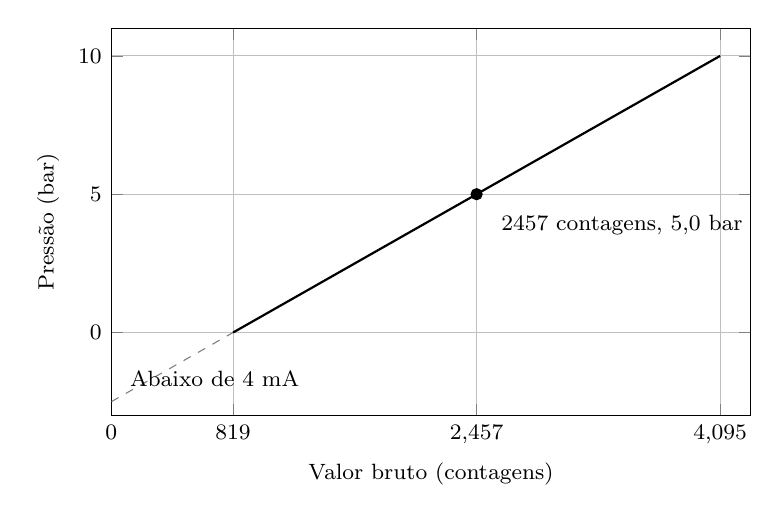
\begin{tikzpicture}
        \begin{axis}[
            width=0.8\textwidth,
            height=6.5cm,
            xlabel={Valor bruto (contagens)},
            ylabel={Pressão (bar)},
            xmin=0, xmax=4300,
            ymin=-3, ymax=11,
            xtick={0,819,2457,4095},
            ytick={0,5,10},
            grid=major,
            tick label style={font=\footnotesize},
            label style={font=\footnotesize}
        ]
            \addplot[gray, dashed, domain=0:819, samples=2] {10/3276*x - 2.5};
            \addplot[thick, domain=819:4095, samples=2] {10/3276*x - 2.5};
            \addplot[only marks, mark=*] coordinates {(2457,5)};
            \node[font=\footnotesize, anchor=north west] at (axis cs:2557,4.6) {2457 contagens, 5{,}0~bar};
            \node[font=\footnotesize, anchor=south west] at (axis cs:60,-2.3) {Abaixo de 4~mA};
        \end{axis}
    \end{tikzpicture}
    \vspace{0.2cm} \\
    Fonte: Autor.
\end{figure}

\par Nem todo sensor ou medidor tem resposta linear. Nos medidores de vazão por pressão diferencial, por exemplo, a vazão é proporcional à raiz quadrada da pressão diferencial medida, de modo que o sinal de 4 a 20\,mA não é proporcional à vazão. A conversão exige a extração da raiz, como na Equação~\ref{eq:cap2_raiz}, em que $Q_\text{max}$ é a vazão de fundo de escala. Com o sinal em 25\,\% da faixa, a vazão calculada é $\sqrt{0{,}25} = 50\,\%$ do fundo de escala, o que mostra por que tratar essa medição como linear levaria a um erro grosseiro.

\myequation{Q = Q_\text{max} \cdot \sqrt{\frac{x - x_\text{min}}{x_\text{max} - x_\text{min}}}}{eq:cap2_raiz}{Vazão a partir do valor bruto de um medidor de pressão diferencial}{\text{u.e.}}

\par Para relações não lineares sem expressão simples, como a conversão do nível de um tanque de geometria irregular em volume, ou a curva de um sensor de temperatura, usa-se a linearização por partes. A curva é descrita por uma tabela de pontos de calibração $(x_i, y_i)$ e, para um valor bruto $x$ situado entre dois pontos consecutivos, a grandeza é obtida por interpolação linear, como na Equação~\ref{eq:cap2_interp}, válida para $x_i \leq x \leq x_{i+1}$. Quanto maior o número de pontos, melhor a aproximação da curva real.

\myequation{y = y_i + \frac{y_{i+1} - y_i}{x_{i+1} - x_i} \cdot (x - x_i)}{eq:cap2_interp}{Interpolação linear entre dois pontos consecutivos de calibração}{\text{u.e.}}

\par Em resumo, o ajuste de escala é a ponte entre o mundo físico, em que a grandeza é medida, e o mundo digital, em que ela é armazenada, exibida e comparada com limites de alarme. Por isso a escala deve ser configurada para cada ponto de forma explícita, e o valor bruto e o valor em unidade de engenharia devem ser distinguidos com clareza, a fim de que um erro de calibração não passe despercebido na operação.

\subsection{Automação e Tecnologias da Indústria 4.0}

\par A automação industrial é o conjunto de tecnologias e práticas que substituem a intervenção humana direta na execução de processos produtivos por sistemas eletrônicos, mecânicos e computacionais capazes de medir, controlar, comandar e supervisionar variáveis físicas. A informática industrial, por sua vez, designa a aplicação das tecnologias da informação e da comunicação a esse contexto, articulando o mundo da \sigla{ta}, voltado a tempo real determinístico, robustez e segurança operacional, com o da \sigla{ti}, orientado a interoperabilidade, escala e segurança da informação. A convergência entre \sigla{ta} e \sigla{ti} é um dos principais vetores de transformação da automação contemporânea \cite{COLOMBO2014_STATE_ART_AUTOMATION}, frequentemente descrita como o desfecho que conduz à Indústria 4.0 \cite{PISCHING2017,BIGHETI2020}.

\par A \sigla{iot} é uma rede global que liga à internet objetos físicos e virtuais, cada um com identidade digital própria, capazes de trocar informações entre si sem intervenção humana \cite{PISCHING2017,BIGHETI2020}. Ela reúne em um mesmo ambiente tecnologias como a computação móvel, as redes de sensores sem fio e os sistemas ciber-físicos, apontando para um cenário em que medir e monitorar o mundo se torna tão corriqueiro quanto o uso da eletricidade \cite{STANKOVIC2014_IOT_RESEARCH_DIRECTIONS}.

\par Quando esse paradigma é levado para o ambiente industrial, sensoriamento de processos, controle de máquinas e otimização da produção, recebe o nome de \sigla{iiot}, um ramo da \sigla{iot} voltado a aumentar a eficiência e a agilidade das fábricas \cite{BIGHETI2020}. Embora partam da mesma base, a \sigla{iot} de consumo e a \sigla{iiot} diferem no grau de criticidade: a de consumo atende a usos casuais e com exigências leves, enquanto a industrial opera com equipamentos fixos, grande volume de dados e requisitos rígidos de resposta em tempo real, confiabilidade e segurança \cite{BIGHETI2020}. A expansão da \sigla{iot} na indústria leva os fabricantes a incorporar tecnologias que sustentam a convergência \sigla{ta}/\sigla{ti} \cite{PISCHING2017}. À medida que os dispositivos de campo passam a oferecer suas funções como serviços de rede, a pirâmide ISA-95 \cite{ISA95_2000_ENTERPRISE_CONTROL} tende a achatar-se em uma arquitetura plana baseada em serviços \cite{COLOMBO2014_STATE_ART_AUTOMATION}.

\par A base de comunicação que sustenta esses conceitos é a troca direta de informações entre dispositivos, denominada \sigla{m2m}. Originada na telemetria industrial e nos primeiros sistemas \sigla{scada}, a \sigla{m2m} precede e fundamenta a \sigla{iot} e viabiliza a noção de máquina inteligente: dispositivos que coordenam ações, ajustam parâmetros e reportam estados sem intervenção manual \cite{BIGHETI2020,PISCHING2017}. Tecnologicamente, apoia-se em uma família de protocolos de comunicação que conectam os equipamentos de campo aos serviços em nuvem, mesmo em redes de longa distância, por meio de modems celulares e \emph{gateways} que concentram as sessões, permitindo supervisionar centenas de pontos remotos sem hardware proprietário em cada instalação \cite{COLOMBO2014_STATE_ART_AUTOMATION}.

\par Os \sigla{cps}, termo proposto em 2006 nos Estados Unidos, descrevem o acoplamento intensivo entre entidades computacionais e o mundo físico \cite{PISCHING2017,MONOSTORI2016_CPS_MANUFACTURING}. A Figura~\ref{fig:cps} ilustra esse acoplamento. Mais do que a soma das partes, é a interseção entre os mundos físico e cibernético que caracteriza o \sigla{cps} \cite{MONOSTORI2016_CPS_MANUFACTURING}. Herdeiros dos sistemas embarcados, os \sigla{cps} acrescentam conectividade, autonomia e cooperação, e no domínio da manufatura recebem o nome de sistemas ciber-físicos de produção. Três características são essenciais aos \sigla{cps} \cite{MONOSTORI2016_CPS_MANUFACTURING}. A inteligência é a capacidade de adquirir informações do entorno e agir de forma autônoma. A conectividade traduz-se no uso de conexões com outros elementos, pessoas e serviços. A responsividade é a reação em tempo apropriado a mudanças. Os \sigla{cps} oferecem a base física e computacional sobre a qual a \sigla{iot} viabiliza a Indústria 4.0 \cite{PISCHING2017}.

\begin{figure}[H]
    \centering
    \caption{Estrutura de um Sistema Ciber-Físico}
    \centering
    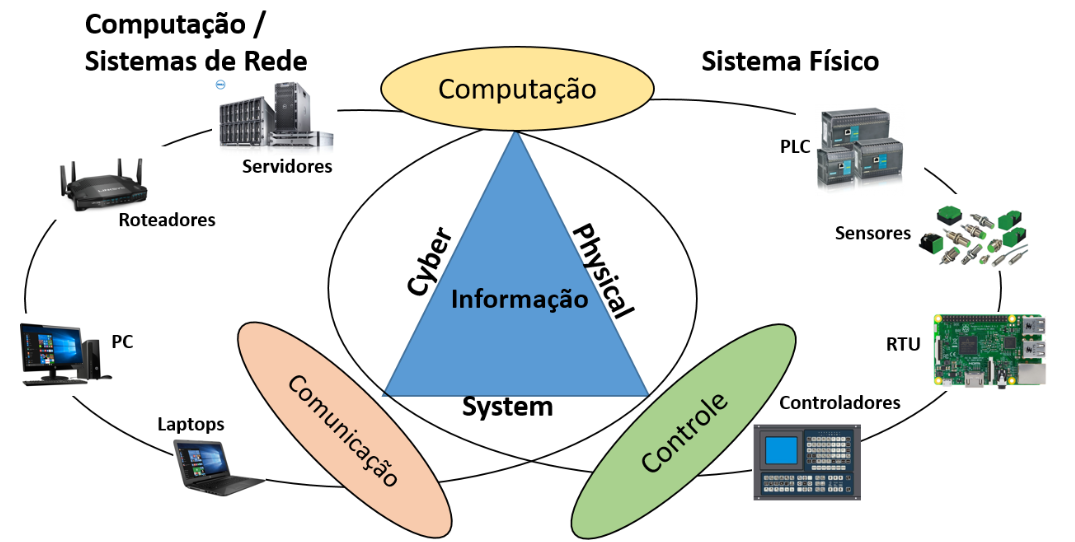
\includegraphics[width=0.85\textwidth]{Imagens/Desenvolvimento/Cap1/cps.png}
    \centering
    \vspace{0.2cm} \\
    Fonte: Adaptado de \textcite{BIGHETI2020}.
    \label{fig:cps}
\end{figure}

\par A Indústria 4.0 nasce do encontro de duas forças. De um lado, a demanda do mercado por produtos personalizados, flexíveis e de produção descentralizada. De outro, o avanço da tecnologia, com mais automação, digitalização e equipamentos cada vez menores \cite{LASI_INDUSTRY_40}. Pode ser entendida como um conjunto de tecnologias coordenadas para conferir competitividade e customização, habilitadas por \sigla{cps}, \sigla{iiot}, computação em nuvem, redes sem fio e uso massivo de dados, cujo conceito-síntese é a fábrica inteligente \cite{BIGHETI2020}. Seus princípios de projeto são a interoperabilidade, a virtualização, a descentralização, a operação em tempo real, a orientação a serviços e a modularidade, padronizados pelo modelo de referência RAMI 4.0 \cite{PISCHING2017}. Nesse contexto, o \sigla{scada} deixa de ser um sistema fechado de supervisão local e passa a um nó de uma rede de serviços que integra produção, manutenção, logística e clientes em uma cadeia de valor digital \cite{BIGHETI2020,COLOMBO2014_STATE_ART_AUTOMATION}. A Figura~\ref{fig:venn_iot_iiot_cps_i40} sintetiza as relações entre esses conceitos: a \sigla{iot} como universo mais amplo, a \sigla{iiot} em sua interseção com o domínio industrial, os \sigla{cps} como categoria de forte acoplamento computação-físico, e a Indústria 4.0 emergindo na interseção entre \sigla{iiot} e \sigla{cps} \cite{BIGHETI2020,PISCHING2017}.

\begin{figure}[H]
    \centering
    \caption{Interseções de IoT, CPS, IIoT e Indústria 4.0}
    \centering
    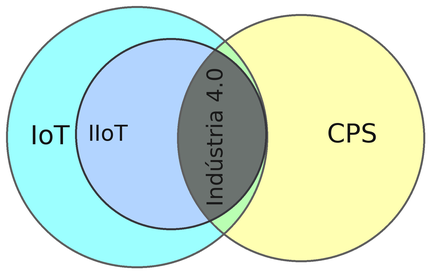
\includegraphics[width=0.65\textwidth]{Imagens/Desenvolvimento/Cap1/venn_iot_iiot_cps.png}
    \centering
    \vspace{0.2cm} \\
    Fonte: \textcite[p.~27]{BIGHETI2020}.
    \label{fig:venn_iot_iiot_cps_i40}
\end{figure}

\subsection{Computação em Nuvem}

\par A Computação em Nuvem é um modelo no qual os dados e as aplicações deixam de residir no computador do usuário e passam a ser executados em grandes centros de processamento e armazenamento, disponibilizados na forma de serviços acessados pela internet \cite{HENRIQUES2010_CLOUD_COMPUTING_TCC}. Em vez de adquirir e manter a própria infraestrutura, o usuário contrata de um provedor a capacidade de processamento, o armazenamento e os programas de que necessita, bastando um dispositivo conectado à rede para utilizá-los \cite{HENRIQUES2010_CLOUD_COMPUTING_TCC}. A ``nuvem'' é a camada conceitual que oculta os equipamentos físicos e os recursos por trás de uma interface padronizada, de modo que a capacidade computacional se apresenta ao usuário como praticamente ilimitada e é provisionada conforme a necessidade \cite{PEDROSA2011_COMPUTACAO_NUVEM,HENRIQUES2010_CLOUD_COMPUTING_TCC}. Para uma plataforma ser de fato uma nuvem, ela precisa reunir cinco características: contratar recursos sozinho e na hora em que precisa, acessar tudo pela rede de qualquer lugar, compartilhar os mesmos recursos entre vários clientes, aumentar ou reduzir a capacidade com rapidez e medir o consumo dos recursos \cite{HENRIQUES2010_CLOUD_COMPUTING_TCC,PEDROSA2011_COMPUTACAO_NUVEM}. Quanto à forma de implantação, a nuvem pode ser pública, privada, comunitária ou híbrida, sendo esta última capaz de recorrer a recursos públicos para absorver picos de demanda \cite{HENRIQUES2010_CLOUD_COMPUTING_TCC}.

\par Os serviços de nuvem costumam ser classificados em três modelos conforme o nível de abstração oferecido. Na infraestrutura como serviço (\emph{Infrastructure as a Service}, IaaS), o usuário contrata máquinas virtuais, armazenamento e redes e administra o que roda sobre eles. Na plataforma como serviço (\emph{Platform as a Service}, PaaS), o provedor também administra o ambiente de execução e o usuário só fornece a aplicação. No \emph{software} como serviço (\emph{Software as a Service}, SaaS), o usuário consome uma aplicação pronta pela internet \cite{HENRIQUES2010_CLOUD_COMPUTING_TCC,PEDROSA2011_COMPUTACAO_NUVEM}. Grandes empresas de tecnologia atuam como provedores desses serviços, como a Amazon, a Microsoft e o Google, e a escolha entre eles é um tema relevante porque a migração de uma aplicação entre provedores diferentes é trabalhosa quando ela depende de serviços proprietários \cite{HENRIQUES2010_CLOUD_COMPUTING_TCC}.

\par Esse modelo traz como principais vantagens a mobilidade de acesso, a dispensa de manter infraestrutura própria, a facilidade de aumentar ou reduzir a capacidade e a confiabilidade dos grandes provedores. Em contrapartida, ainda apresenta desafios, como a segurança dos dados, a dificuldade de migrar entre provedores diferentes e a garantia de disponibilidade \cite{HENRIQUES2010_CLOUD_COMPUTING_TCC,PEDROSA2011_COMPUTACAO_NUVEM}. No contexto da Indústria 4.0, a nuvem funciona como a infraestrutura que conecta produtos, máquinas, sensores e serviços, e passa a tratar o \sigla{scada}, antes restrito a salas de controle locais, como mais um ponto de uma rede distribuída de serviços \cite{BIGHETI2020,PISCHING2017}.

\subsection{Contêineres e Orquestração}

\par A virtualização é a tecnologia que abstrai os recursos físicos de um sistema de computação para oferecer um ambiente computacional virtual, de modo a melhorar o aproveitamento dos recursos disponíveis \cite{NETTO2017_COORDENACAO_CONTAINERS_KUBERNETES}. Na forma tradicional, a virtualização ocorre por meio de máquinas virtuais, ambientes de software construídos sobre as interfaces dos recursos físicos, em que cada máquina executa um sistema operacional completo, chamado de convidado, sob o controle de um monitor de máquinas virtuais, também denominado hipervisor \cite{NETTO2017_COORDENACAO_CONTAINERS_KUBERNETES}. Esse modelo, predominante nos centros de dados que sustentam a computação em nuvem, oferece forte isolamento entre as cargas de trabalho, mas cada máquina carrega o custo de um sistema operacional inteiro \cite{NETTO2016_STATE_MACHINE_REPLICATION_KUBERNETES}.

\par A virtualização baseada em contêineres propõe uma alternativa mais leve. Em vez de virtualizar o hardware, o contêiner virtualiza o próprio sistema operacional: ele compartilha o núcleo do sistema hospedeiro e isola os seus processos dos demais processos em execução, cabendo a um gerenciador de contêineres mediar o uso dos recursos \cite{NETTO2017_COORDENACAO_CONTAINERS_KUBERNETES}. A ideia tem origem em mecanismos como o comando \emph{jail}, do sistema FreeBSD, e as \emph{zones}, do sistema Solaris, e se difundiu com o Linux, cujo núcleo oferece os recursos de isolamento e de limitação de consumo de processador e memória sobre os quais os contêineres atuais se apoiam \cite{NETTO2017_COORDENACAO_CONTAINERS_KUBERNETES,DOCKER_DOCS}. A Figura~\ref{fig:cap2_vm_conteiner} compara os dois modelos.

\begin{figure}[H]
    \centering
    \caption{Máquinas virtuais e contêineres}
    \label{fig:cap2_vm_conteiner}
    \vspace{0.4cm}
    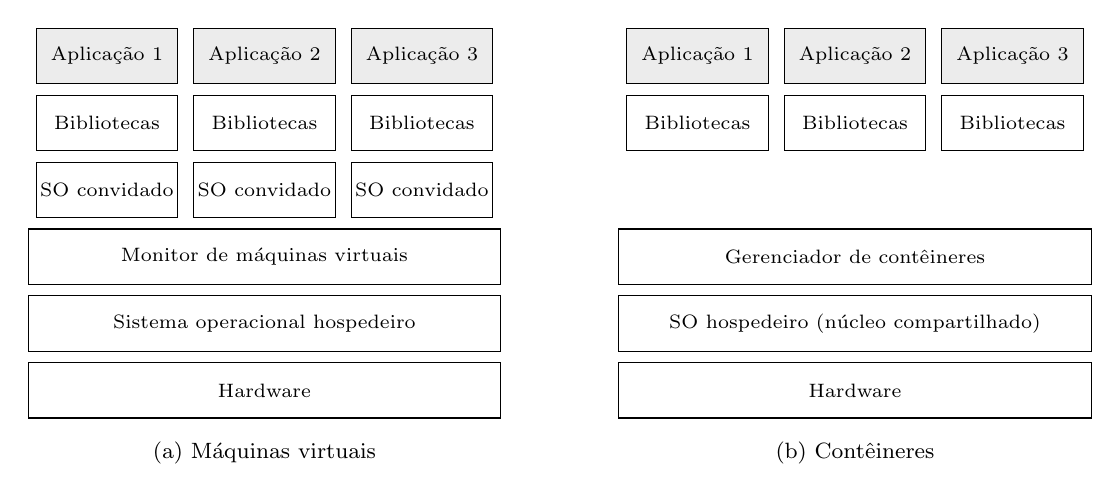
\begin{tikzpicture}[
        caixa/.style={draw, rectangle, minimum height=0.7cm, font=\scriptsize, align=center, inner sep=1pt},
        larga/.style={caixa, minimum width=6cm},
        estreita/.style={caixa, minimum width=1.8cm}
    ]
        \node[larga] at (3,0.35) {Hardware};
        \node[larga] at (3,1.2) {Sistema operacional hospedeiro};
        \node[larga] at (3,2.05) {Monitor de máquinas virtuais};
        \foreach \x/\n in {1/1,3/2,5/3} {
            \node[estreita] at (\x,2.9) {SO convidado};
            \node[estreita] at (\x,3.75) {Bibliotecas};
            \node[estreita, fill=gray!15] at (\x,4.6) {Aplicação \n};
        }
        \node[font=\footnotesize] at (3,-0.45) {(a) Máquinas virtuais};

        \begin{scope}[xshift=7.5cm]
            \node[larga] at (3,0.35) {Hardware};
            \node[larga] at (3,1.2) {SO hospedeiro (núcleo compartilhado)};
            \node[larga] at (3,2.05) {Gerenciador de contêineres};
            \foreach \x/\n in {1/1,3/2,5/3} {
                \node[estreita] at (\x,3.75) {Bibliotecas};
                \node[estreita, fill=gray!15] at (\x,4.6) {Aplicação \n};
            }
            \node[font=\footnotesize] at (3,-0.45) {(b) Contêineres};
        \end{scope}
    \end{tikzpicture}
    \vspace{0.2cm} \\
    Fonte: Elaborado pelo autor com base em \textcite{NETTO2017_COORDENACAO_CONTAINERS_KUBERNETES}.
\end{figure}

\par Como o contêiner não precisa inicializar um sistema operacional próprio, ele é instanciado e recebe seus recursos de forma muito mais rápida que uma máquina virtual, e a aplicação só consome recursos enquanto o contêiner está em execução \cite{NETTO2017_COORDENACAO_CONTAINERS_KUBERNETES}. O contêiner é criado a partir de uma imagem, um pacote estático e imutável que reúne a aplicação, suas bibliotecas e dependências, normalmente construído em camadas, de modo que apenas os arquivos que ainda não existem no sistema hospedeiro ocupam espaço adicional \cite{NETTO2016_STATE_MACHINE_REPLICATION_KUBERNETES}. Essa característica garante portabilidade, pois a mesma imagem executa de forma idêntica no computador do desenvolvedor, em um servidor local ou em um provedor de nuvem. Em contrapartida, como as imagens são estáticas, o contêiner é essencialmente um ambiente sem estado, e tanto o estado do contêiner quanto o das aplicações que nele executavam se perdem quando ele é encerrado, a menos que os dados sejam gravados em volumes externos \cite{NETTO2017_COORDENACAO_CONTAINERS_KUBERNETES}.

\par O Docker é a ferramenta de contêineres mais difundida. Ele oferece o formato de imagem, a descrição declarativa da construção da imagem em um arquivo de receita, o registro onde as imagens são armazenadas e distribuídas e o motor que executa os contêineres \cite{DOCKER_DOCS}. Para aplicações formadas por vários contêineres que precisam trabalhar juntos, uma aplicação com servidor web, banco de dados e serviços de apoio, por exemplo, a ferramenta Docker Compose descreve em um único arquivo os contêineres, as redes que os conectam e os volumes que guardam seus dados, o que permite subir todo o conjunto com um comando \cite{DOCKER_DOCS}. Contudo, a implementação nativa do Docker não oferece mecanismos de gerenciamento, orquestração e integração de contêineres em um agrupamento de máquinas (\emph{cluster}), requisito desejável para a tolerância a faltas \cite{NETTO2017_COORDENACAO_CONTAINERS_KUBERNETES}.

\par A orquestração de contêineres é a automação do ciclo de vida de muitos contêineres distribuídos em várias máquinas. O orquestrador mais difundido é o Kubernetes, criado pelo Google a partir da experiência com o sistema interno Borg e entregue à \emph{Cloud Native Computing Foundation}, fundação criada para orientar a adoção de contêineres em nuvem de maneira padronizada \cite{NETTO2016_STATE_MACHINE_REPLICATION_KUBERNETES,KUBERNETES_DOCS}. Suas principais funcionalidades são o controle de admissão dos contêineres, o balanceamento de recursos entre as máquinas, a descoberta de serviços, a publicação de um serviço para acessos externos ao agrupamento e o balanceamento da carga entre as réplicas de um contêiner \cite{NETTO2017_COORDENACAO_CONTAINERS_KUBERNETES}.

\par A arquitetura do Kubernetes é composta por máquinas, físicas ou virtuais, denominadas nós. A unidade básica de gerenciamento é o \emph{pod}, que abriga um ou mais contêineres fortemente acoplados, os quais compartilham recursos como volumes e endereço de rede. Cada nó executa um agente, o \emph{kubelet}, que gerencia os \emph{pods} e informa o estado dos contêineres ao nó principal, e um \emph{proxy}, que recebe as requisições e as encaminha aos \emph{pods}, distribuindo a carga entre as réplicas, por exemplo pelo critério \emph{round robin}. O nó principal reúne os componentes de gerenciamento, o servidor de API, pelo qual os demais componentes e o operador interagem com o agrupamento, e o armazenamento distribuído \emph{etcd}, onde as informações do agrupamento são persistidas \cite{NETTO2017_COORDENACAO_CONTAINERS_KUBERNETES,NETTO2016_STATE_MACHINE_REPLICATION_KUBERNETES}. O Kubernetes replica contêineres para aumentar a disponibilidade, e quando um contêiner falha ele o recria a partir da imagem \cite{NETTO2016_STATE_MACHINE_REPLICATION_KUBERNETES}. Esses recursos de escalonamento, réplicas, descoberta de serviços e recuperação de falhas permitem tratar um conjunto de máquinas como uma única plataforma de execução, na qual a aplicação declara quantas réplicas deseja e o orquestrador trabalha para manter esse estado.

\par O Kubernetes, porém, replica contêineres e não o estado das aplicações neles hospedadas, pois o contêiner recriado volta ao estado da imagem. Usar volumes externos mitiga o problema, mas exige que o volume seja protegido contra falhas e que a aplicação controle os acessos concorrentes a ele \cite{NETTO2016_STATE_MACHINE_REPLICATION_KUBERNETES}. Para aplicações que alteram um estado e precisam tolerar a falha de réplicas, uma abordagem consolidada é a replicação de máquinas de estados (\emph{State Machine Replication}, \sigla{smr}), técnica que mantém um conjunto de computadores sincronizados no mesmo estado apesar das faltas que ocorram no sistema \cite{NETTO2019_RAFT_KUBERNETES}. Para tolerar até $f$ faltas por parada, o sistema precisa de pelo menos $n \geq 2f + 1$ réplicas. A técnica se apoia em três propriedades: todas as réplicas corretas partem do mesmo estado inicial, as operações são determinísticas, de modo que a mesma entrada sobre o mesmo estado produz a mesma saída e o mesmo novo estado, e todas as réplicas processam a mesma sequência de comandos \cite{NETTO2019_RAFT_KUBERNETES}. A terceira propriedade, a coordenação, exige que todo pedido seja entregue às réplicas na mesma ordem, o que se obtém com um protocolo de difusão atômica ou de consenso distribuído, equivalentes entre si \cite{NETTO2019_RAFT_KUBERNETES,NETTO2017_COORDENACAO_CONTAINERS_KUBERNETES}.

\par O Raft é um algoritmo de consenso que pode ser usado para implementar a replicação de máquinas de estados, concebido para ser mais fácil de compreender que o Paxos, algoritmo de consenso mais conhecido \cite{ONGARO2014_RAFT,NETTO2019_RAFT_KUBERNETES}. No Raft, uma réplica atua como líder e as demais como seguidoras. As atualizações do estado replicado fluem apenas do líder para os seguidores, o que simplifica o gerenciamento do registro replicado, e por isso somente o líder aceita pedidos dos clientes. A operação normal ocorre em fases, ilustradas na Figura~\ref{fig:cap2_raft}. O cliente envia o pedido ao líder (1), que define a ordem do pedido e o propõe aos seguidores (2). Os seguidores aceitam a proposta e respondem ao líder (3). Quando a maioria aceitou, o líder confirma o pedido e responde ao cliente (4) e, na mensagem seguinte, informa a confirmação aos seguidores, que também a efetivam (5) \cite{NETTO2019_RAFT_KUBERNETES}.

\begin{figure}[H]
    \centering
    \caption{Operação normal do protocolo Raft}
    \label{fig:cap2_raft}
    \vspace{0.4cm}
    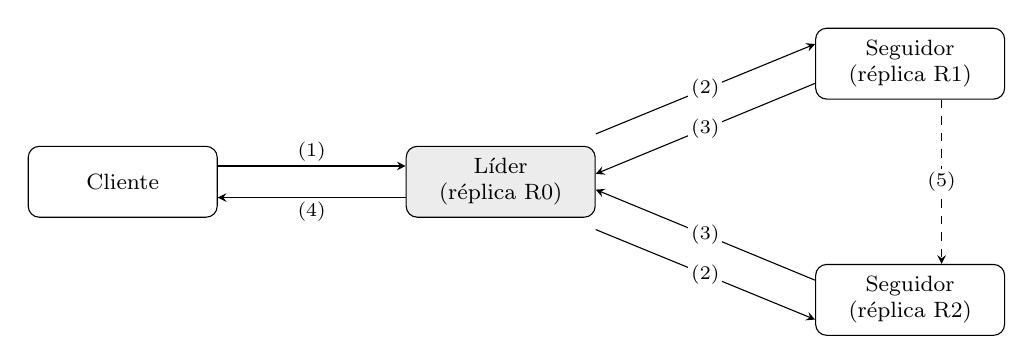
\begin{tikzpicture}[
        caixa/.style={draw, rectangle, rounded corners, minimum width=2.4cm, minimum height=0.9cm, font=\footnotesize, align=center},
        seta/.style={->, >=stealth},
        rot/.style={font=\scriptsize, fill=white, inner sep=1pt}
    ]
        \node[caixa] (cli) at (0,0) {Cliente};
        \node[caixa, fill=gray!15] (lid) at (4.8,0) {Líder\\(réplica R0)};
        \node[caixa] (s1) at (10,1.5) {Seguidor\\(réplica R1)};
        \node[caixa] (s2) at (10,-1.5) {Seguidor\\(réplica R2)};
        \draw[seta] ([yshift=0.2cm]cli.east) -- node[rot, above=0.5pt] {(1)} ([yshift=0.2cm]lid.west);
        \draw[seta] ([yshift=-0.2cm]lid.west) -- node[rot, below=0.5pt] {(4)} ([yshift=-0.2cm]cli.east);
        \draw[seta] ([yshift=0.15cm]lid.north east) -- node[rot, pos=0.5] {(2)} ([yshift=0.25cm]s1.west);
        \draw[seta] ([yshift=-0.15cm]lid.south east) -- node[rot, pos=0.5] {(2)} ([yshift=-0.25cm]s2.west);
        \draw[seta] ([yshift=-0.25cm]s1.west) -- node[rot, pos=0.5] {(3)} ([yshift=0.1cm]lid.east);
        \draw[seta] ([yshift=0.25cm]s2.west) -- node[rot, pos=0.5] {(3)} ([yshift=-0.1cm]lid.east);
        \draw[seta, dashed] ([xshift=0.4cm]s1.south) -- node[rot] {(5)} ([xshift=0.4cm]s2.north);
    \end{tikzpicture}
    \vspace{0.2cm} \\
    Fonte: Elaborado pelo autor com base em \textcite{NETTO2019_RAFT_KUBERNETES}.
\end{figure}

\par Se uma réplica não recebe comunicação do líder, nem pelas mensagens periódicas de batimento (\emph{heartbeat}) nem por novos pedidos ordenados, ela se torna candidata e inicia uma eleição, solicitando votos às demais. O novo líder é aquele aceito pela maioria das réplicas. O uso de temporizadores aleatórios nas eleições resolve conflitos de forma simples e rápida e combina com a estratégia do Kubernetes, em que os contêineres não são diferenciados entre si e qualquer um pode se tornar líder. O Raft também usa o conceito de quórum, a maioria das réplicas, para manter o funcionamento durante as trocas de configuração \cite{NETTO2019_RAFT_KUBERNETES}. O próprio \emph{etcd} do Kubernetes é uma implementação desse protocolo \cite{NETTO2019_RAFT_KUBERNETES}.

\par Há ao menos três maneiras de incorporar a coordenação das réplicas a um ambiente existente, a integração, em que um componente do ambiente é construído ou modificado para oferecer a funcionalidade, a interceptação, em que as mensagens destinadas à aplicação são capturadas e mapeadas em um sistema de comunicação de grupo, e o serviço, em que uma camada de software entre o cliente e a aplicação se encarrega de coordenar os pedidos \cite{NETTO2017_COORDENACAO_CONTAINERS_KUBERNETES}. Cada uma dessas abordagens foi explorada para o Kubernetes. A integração, usando o \emph{etcd} como memória compartilhada para guiar a coordenação, foi avaliada experimentalmente e mostrou-se viável \cite{NETTO2016_STATE_MACHINE_REPLICATION_KUBERNETES}. A abordagem baseada em serviço acopla a coordenação à aplicação de maneira leve e simples, e foi avaliada com aplicações de consistência forte e de consistência eventual \cite{NETTO2017_COORDENACAO_CONTAINERS_KUBERNETES}. A incorporação do Raft em contêineres gerenciados pelo Kubernetes, por sua vez, adaptou o algoritmo para a descoberta automática das réplicas e para o encaminhamento ao líder dos pedidos recebidos por seguidores, e a avaliação mostrou desempenho próximo ao do Raft executado em máquinas físicas, com maior consumo de rede na versão em contêineres e maior consumo de processamento e memória na versão em máquinas físicas \cite{NETTO2019_RAFT_KUBERNETES}.

\par Em síntese, os contêineres tornam a implantação leve, portátil e repetível, e os orquestradores adicionam escalonamento, réplicas, descoberta de serviços e recuperação automática de falhas. Quando a tolerância a falhas deve alcançar também o estado das aplicações, a replicação de máquinas de estados com protocolos de consenso como o Raft complementa essa base. Essa decomposição do software em pequenas unidades independentes, executadas e replicadas em contêineres, é o terreno sobre o qual se desenvolve o estilo arquitetural discutido a seguir.

\subsection{Microsserviços}

\par O paradigma de microsserviços é um estilo arquitetural em que a aplicação é estruturada como um conjunto de serviços pequenos, autônomos e independentemente implantáveis, cada um responsável por um domínio bem delimitado e comunicando-se por protocolos leves, tipicamente APIs \sigla{http}/\sigla{rest} ou mensageria assíncrona. O estilo é herdeiro da \sigla{soa}, que organiza as funcionalidades como serviços passíveis de serem publicados, descobertos e consumidos sob demanda \cite{PISCHING2017}, mas distingue-se da \sigla{soa} clássica pela granularidade e pela autonomia, ao adotar serviços pequenos, com bancos próprios e ciclos de vida independentes, em vez de serviços grandes orquestrados por um barramento central \cite{COLOMBO2014_STATE_ART_AUTOMATION}.

\par Esse modelo supera limitações do monolito, em que todas as responsabilidades vivem em um único processo e a escalabilidade aplica-se ao todo, não à parte realmente sobrecarregada. Suas vantagens centrais são a implantação independente, a escalabilidade granular, na qual se replica apenas o gargalo, e a heterogeneidade tecnológica, em que cada serviço usa a linguagem e o banco mais adequados \cite{BIGHETI2020}. No contexto da Indústria 4.0, esses serviços alinham-se aos princípios de modularidade, descentralização e orientação a serviços \cite{PISCHING2017,BIGHETI2020}.

\subsection{Moleculer}

\par O Moleculer é uma ferramenta para a construção de microsserviços na plataforma Node.js, voltada a sistemas distribuídos formados por serviços pequenos e independentes \cite{MOLECULER_DOCS}. Em uma única biblioteca leve, reúne os recursos necessários para que esses serviços se localizem na rede, dividam a carga de trabalho entre si e continuem operando diante de falhas, o que a torna uma alternativa mais simples a soluções mais complexas \cite{MOLECULER_DOCS}.

\par Cada serviço expõe um conjunto de operações que podem ser chamadas remotamente por outros serviços, e também envia avisos quando algo relevante acontece, para que os demais serviços reajam. Cada serviço registra-se em um componente central de coordenação, responsável por localizar automaticamente os serviços disponíveis e encaminhar cada chamada à cópia mais adequada, distribuindo o trabalho entre as cópias em execução \cite{MOLECULER_DOCS}. Quando uma dessas cópias falha, esse coordenador redireciona a chamada para outra ou devolve uma resposta alternativa, evitando que a falha de um único serviço se propague pelo restante do sistema. Essa capacidade de manter o funcionamento mesmo diante de falhas alinha-se às arquiteturas de microsserviços empregadas na Indústria 4.0 \cite{BIGHETI2020}.

\subsection{Filas de Mensagens e Processamento Assíncrono}

\par Uma fila de mensagens é uma estrutura intermediária que desacopla quem solicita um trabalho de quem o executa. O componente que cria a mensagem, chamada de tarefa ou \emph{job}, e a insere na fila é o produtor. O componente que retira as mensagens e as processa é o consumidor, frequentemente chamado de \emph{worker}. Como produtor e consumidor não precisam estar disponíveis ao mesmo tempo nem operar no mesmo ritmo, o processamento passa a ser assíncrono: o produtor registra o pedido e segue adiante sem esperar o resultado, enquanto o consumidor o atende quando houver capacidade \cite{BULLMQ_DOCS}.

\par Esse arranjo traz benefícios. A fila absorve picos de demanda, pois as tarefas excedentes esperam em vez de sobrecarregar o consumidor. Permite escalar o processamento de forma independente, bastando acrescentar consumidores para drenar a fila mais depressa. Isola falhas, já que a indisponibilidade momentânea do consumidor não impede o produtor de registrar novas tarefas. E retira do caminho de uma requisição interativa os trabalhos demorados, de modo que o usuário recebe a resposta sem aguardar a conclusão do trabalho \cite{BULLMQ_DOCS}.

\par A confiabilidade do processamento assíncrono depende de algumas práticas. As filas costumam entregar cada tarefa ao menos uma vez, o que significa que uma mesma tarefa pode ser executada mais de uma vez, por exemplo quando um consumidor falha antes de confirmar a conclusão. Por isso o tratamento da tarefa deve ser idempotente, isto é, executá-lo duas vezes deve produzir o mesmo resultado que executá-lo uma vez. Gravar um registro com uma chave única, ou atualizar um valor para um estado final em vez de somá-lo a um acumulado, são formas usuais de obter idempotência. Quando o tratamento falha, a fila repete a tarefa por um número limitado de tentativas, com espera crescente entre elas (\emph{backoff}), para não sobrecarregar um recurso que ainda se recupera. Há falhas que não se resolvem repetindo, como um dado inválido, e para elas a tarefa deve ser encerrada de imediato e movida para uma fila de mensagens mortas (\emph{dead-letter}), onde permanece disponível para análise. Convém também limitar a concorrência de cada consumidor, atribuir prioridades, manter o conteúdo da mensagem pequeno, com identificadores em vez de dados completos, e limpar periodicamente as tarefas concluídas para que a fila não cresça sem limite \cite{BULLMQ_DOCS}. A Figura~\ref{fig:cap2_fila} resume o fluxo.

\begin{figure}[H]
    \centering
    \caption{Fluxo de uma fila de mensagens com tentativas e fila de mensagens mortas}
    \label{fig:cap2_fila}
    \vspace{0.4cm}
    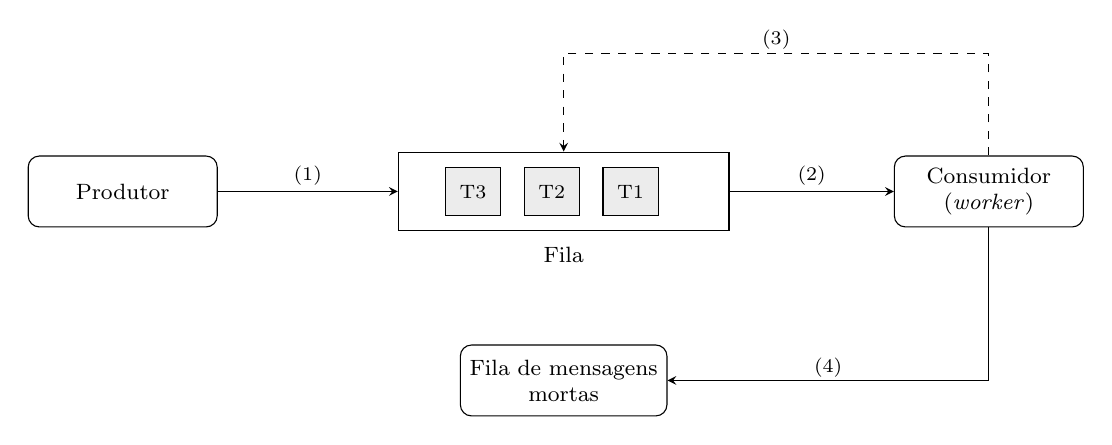
\begin{tikzpicture}[
        caixa/.style={draw, rectangle, rounded corners, minimum width=2.4cm, minimum height=0.9cm, font=\footnotesize, align=center},
        msg/.style={draw, rectangle, minimum width=0.7cm, minimum height=0.6cm, font=\scriptsize, fill=gray!15},
        seta/.style={->, >=stealth},
        rot/.style={font=\scriptsize, fill=white, inner sep=1pt}
    ]
        \node[caixa] (prod) at (0,0) {Produtor};
        \node[draw, rectangle, minimum width=4.2cm, minimum height=1cm] (fila) at (5.6,0) {};
        \node[font=\footnotesize] at (5.6,-0.8) {Fila};
        \node[msg] at (4.45,0) {T3};
        \node[msg] at (5.45,0) {T2};
        \node[msg] at (6.45,0) {T1};
        \node[caixa] (cons) at (11,0) {Consumidor\\(\emph{worker})};
        \node[caixa] (morta) at (5.6,-2.4) {Fila de mensagens\\mortas};
        \draw[seta] (prod.east) -- node[rot, above=1pt] {(1)} (fila.west);
        \draw[seta] (fila.east) -- node[rot, above=1pt] {(2)} (cons.west);
        \draw[seta, dashed] (cons.north) -- ++(0,1.3) -| node[rot, pos=0.25, above] {(3)} (fila.north);
        \draw[seta] (cons.south) |- node[rot, pos=0.75, above] {(4)} (morta.east);
    \end{tikzpicture}
    \vspace{0.2cm} \\
    Fonte: Autor.
\end{figure}

\par A figura mostra o caminho de uma tarefa. O produtor insere a tarefa na fila (1) e o consumidor a retira e a processa (2). Se o processamento falha e ainda restam tentativas, a tarefa retorna à fila após a espera definida (3). Esgotadas as tentativas, ou diante de uma falha sem solução, a tarefa é movida para a fila de mensagens mortas (4).

\par O BullMQ é uma biblioteca de filas para a plataforma Node.js que guarda o estado das filas no Redis. Ela oferece tentativas com \emph{backoff}, tarefas com atraso, tarefas repetíveis agendadas por expressões de tempo, prioridades, limite de concorrência e de taxa, e a remoção automática de tarefas concluídas e falhadas segundo critérios de idade e de quantidade \cite{BULLMQ_DOCS}. Como todo o estado da fila reside no Redis, a configuração desse banco influi na confiabilidade do conjunto. Em particular, uma política de memória que descarte chaves quando o limite é atingido pode eliminar tarefas em silêncio, razão pela qual recomenda-se a política que recusa novas escritas, em vez de remover dados existentes, quando a memória se esgota \cite{REDIS_DOCS,BULLMQ_DOCS}.

\subsection{Banco de Dados}

\par O banco de dados é o componente de software responsável por armazenar, organizar e recuperar informações de forma persistente. Quanto à organização dos dados, destacam-se dois grandes paradigmas: o relacional, que estrutura os dados em tabelas com esquema definido e relações explícitas entre as entidades, e o NoSQL, voltado a cenários de alta variabilidade de esquema e escala horizontal \cite{MOHAMED2014_RELATIONAL_VS_NOSQL}. Por organizar os dados de forma estruturada e preservar a integridade entre entidades relacionadas, o modelo relacional é o adequado a sistemas que exigem consistência e consultas expressivas, sendo o detalhado a seguir.

\par O modelo relacional, materializado em bancos como PostgreSQL, MySQL e Oracle, organiza os dados em tabelas de linhas e colunas, cada uma definida por um esquema, uma chave primária que identifica unicamente cada registro e, opcionalmente, chaves estrangeiras que estabelecem relações entre tabelas, garantindo integridade referencial \cite{MOHAMED2014_RELATIONAL_VS_NOSQL}. A linguagem de consulta padrão é o \sigla{sql} (\emph{Structured Query Language}), com operações de seleção, inserção, atualização e remoção, além de junções, agregações, transações e índices.

\par Em ambientes de produção, boas práticas incluem indexar os campos mais consultados, particionar as tabelas históricas por intervalo de tempo para evitar tabelas monolíticas e empregar réplicas que assumem o serviço automaticamente quando o nó principal falha e cópias do estado do banco em pontos definidos no tempo para alta disponibilidade.

\par O particionamento de tabelas divide uma tabela lógica muito grande em partes físicas menores, as partições, segundo um critério como o intervalo de valores de uma coluna. Para dados históricos que crescem continuamente, como medições coletadas ao longo do tempo, o critério natural é o intervalo de tempo, com uma partição por mês, por exemplo. O planejador de consultas ignora as partições que não podem conter os registros pedidos, técnica denominada poda de partições, e por isso uma consulta sobre um período recente varre apenas as partições correspondentes. A remoção de dados antigos também fica mais barata, pois descartar uma partição inteira é muito mais rápido que apagar milhões de linhas uma a uma e evita a fragmentação do armazenamento \cite{POSTGRESQL_DOCS}. Associado ao particionamento, é usual manter tabelas de agregados pré-calculados, como as médias por minuto ou por hora, que permitem exibir longos períodos sem percorrer todos os registros brutos.

\par Em sistemas que atendem várias organizações clientes, chamados multi-inquilino (\emph{multi-tenant}), existem três estratégias principais de organização dos dados. Na primeira, todos os clientes compartilham o mesmo banco e as mesmas tabelas, e uma coluna identifica o inquilino dono de cada linha. Na segunda, cada cliente tem seu próprio esquema dentro de um banco compartilhado. Na terceira, cada cliente tem um banco de dados dedicado \cite{CHONG2006_MULTITENANT}. As duas primeiras favorecem o custo e a densidade de clientes por servidor, mas dependem de filtros corretos em toda consulta para evitar a exposição de dados entre clientes. O banco dedicado oferece o isolamento mais forte, permite fazer cópias de segurança, restaurar e excluir os dados de um cliente de modo independente e até hospedá-los em um servidor escolhido por ele, ao custo de mais conexões abertas, de mais bancos a administrar e de migrações de esquema que precisam ser aplicadas a cada banco \cite{CHONG2006_MULTITENANT}.

\subsection{Redis}

\par O \emph{Redis} é um armazenamento de dados em memória, de código aberto, que opera como banco chave-valor de altíssimo desempenho. Diferentemente dos bancos relacionais, em que a persistência em disco é a prioridade, o Redis mantém todo o conjunto de trabalho em memória \sigla{ram}, oferecendo latências sub-milissegundo para operações de leitura e escrita  \cite{REDIS_DOCS}.

\par O Redis oferece persistência opcional por snapshots periódicos e log de operações de escrita, expiração automática de chaves por \sigla{ttl} e um mecanismo publicador-assinante (Pub/Sub) para troca de mensagens entre processos. Por essas características, é comumente empregado como cache de acesso rápido, como barramento de eventos e como armazenamento de dados temporários \cite{REDIS_DOCS}.

\par Como o Redis guarda os dados em memória, ele usa cópias e recuperação automática para não parar diante de falhas. A replicação mantém uma ou mais réplicas sempre atualizadas da instância principal. Sobre isso, o \emph{Redis Sentinel} cuida da disponibilidade: vigia a instância principal e, se ela cai, promove sozinho uma réplica ao seu lugar, sem intervenção manual. Já o \emph{Redis Cluster} cuida do crescimento: reparte as chaves entre vários nós, de modo que basta acrescentar nós para aumentar a capacidade, e cada nó pode ter réplicas para o serviço continuar mesmo se um deles falhar \cite{REDIS_DOCS}.

\par Além de simples pares de texto, o Redis oferece estruturas de dados como listas, conjuntos, conjuntos ordenados e \emph{hashes}, com operações atômicas sobre cada uma, e permite executar pequenos programas na linguagem Lua no próprio servidor, o que garante que uma sequência de comandos seja executada sem interferência de outros clientes \cite{REDIS_DOCS}. Essas características o tornam adequado para guardar o valor mais recente de uma informação que muda com frequência, aplicar limites de taxa de requisições, implementar travas distribuídas entre processos e servir de base para filas, como visto anteriormente.

\subsection{Node.js, TypeScript e Fastify}

\par O Node.js é um ambiente de execução que permite rodar JavaScript fora do navegador, construído sobre o motor V8. Seu modelo de execução é orientado a eventos, com operações de entrada e saída não bloqueantes: um único fluxo de execução atende muitas conexões simultâneas, pois, enquanto uma operação de rede ou de disco aguarda, o laço de eventos processa outras requisições \cite{NODEJS_DOCS}. Esse modelo é adequado a servidores com grande volume de operações de entrada e saída, como APIs e serviços que se comunicam com bancos de dados e com a rede. Em contrapartida, cálculos longos que ocupam o processador bloqueiam o laço de eventos e atrasam todas as demais requisições, razão pela qual esse tipo de trabalho deve ser transferido para processos ou fluxos de execução separados \cite{NODEJS_DOCS}.

\par O TypeScript é um superconjunto do JavaScript que acrescenta um sistema de tipos estáticos. O compilador verifica a coerência dos tipos antes da execução e, em seguida, gera código JavaScript comum, de modo que erros como o uso de um campo inexistente ou a passagem de um argumento de tipo errado são detectados no desenvolvimento, e não em produção \cite{TYPESCRIPT_DOCS}. Os tipos, contudo, existem apenas em tempo de compilação e são apagados na execução. Dados que chegam de fora do programa, como o corpo de uma requisição, não têm garantia de corresponder ao tipo declarado, e por isso precisam ser validados nas fronteiras do sistema.

\par O Fastify é um \emph{framework} web para Node.js voltado a baixo custo computacional por requisição e boa experiência de desenvolvimento. Sua estrutura se baseia em plugins encapsulados, em que cada conjunto de rotas, de configurações e de dependências é registrado em um contexto próprio, o que favorece a organização do código em módulos. O ciclo de vida de cada requisição é dividido em etapas nas quais se podem inserir ganchos (\emph{hooks}), como a autenticação, a validação e o tratamento de erros, e o \emph{framework} permite descrever o formato esperado da requisição e da resposta por meio de esquemas, usados tanto para validar a entrada quanto para serializar a saída com eficiência \cite{FASTIFY_DOCS}.

\par A validação de contratos por esquema é a técnica que descreve, de forma declarativa, a estrutura que os dados devem ter, e rejeita o que não a respeita. A biblioteca Zod, desenvolvida para o TypeScript, permite declarar esse esquema em código e dele inferir automaticamente o tipo estático correspondente, de modo que um único artefato serve como validação em tempo de execução e como tipo em tempo de compilação \cite{ZOD_DOCS}. Quando o esquema é compartilhado entre o servidor e o cliente, ambos concordam sobre o formato das mensagens e uma divergência, como a remoção de um campo, é detectada na compilação. Os esquemas também podem ser usados para gerar a documentação da API, mantendo-a sincronizada com o comportamento real \cite{ZOD_DOCS,FASTIFY_DOCS}.

\subsection{React e Next.js}

\par O React é uma biblioteca JavaScript, desenvolvida pela Meta, para montar interfaces de usuário a partir de componentes, isto é, pequenos blocos reutilizáveis de tela, como botões, formulários e gráficos, que se combinam para formar páginas inteiras. Sua abordagem é declarativa: o desenvolvedor descreve como a interface deve ser para um dado estado da aplicação, e o React se encarrega de atualizar apenas as partes da tela que mudaram quando o estado muda, comparando a nova descrição com a anterior em uma representação intermediária em memória \cite{REACT_DOCS}. Os componentes recebem dados por propriedades e mantêm estado interno por meio de ganchos (\emph{hooks}), e a composição de componentes pequenos facilita o reaproveitamento e o teste \cite{REACT_DOCS}.

\par O Next.js é um \emph{framework} para a construção de aplicações web criado sobre o React. O React, sozinho, monta a interface diretamente no navegador do usuário: envia um arquivo quase vazio acompanhado de um programa em JavaScript que desenha a tela depois que a página carrega. Esse modelo, chamado de renderização no cliente, funciona bem, mas tem desvantagens, a primeira carga pode ser lenta e os mecanismos de busca têm dificuldade para ler o conteúdo \cite{NEXTJS_DOCS}.

\par O Next.js surge justamente para contornar essas limitações, oferecendo outras formas de gerar as páginas. Na renderização no servidor, a página já é montada por completo antes de ser enviada ao navegador, o que acelera a exibição e facilita a leitura pelos buscadores. Na geração estática, a página é montada uma única vez, no momento em que o sistema é publicado, e a mesma versão pronta é entregue a todos os usuários, garantindo o melhor desempenho para conteúdos que mudam pouco. Uma vantagem importante é que o Next.js permite escolher a estratégia mais adequada para cada tela, em vez de impor uma só a toda a aplicação \cite{NEXTJS_DOCS}.

\par Além das opções de renderização, o Next.js simplifica tarefas comuns do desenvolvimento. O roteamento, isto é, a associação entre os endereços e as páginas, baseia-se na própria organização dos arquivos do projeto: cada arquivo criado em uma pasta específica vira automaticamente um endereço da aplicação, sem necessidade de configuração manual. O \emph{framework} ainda traz, de fábrica, recursos que melhoram o desempenho, como carregar apenas o código necessário a cada página, preparar de antemão as páginas que o usuário provavelmente acessará, otimizar imagens automaticamente e oferecer suporte nativo ao TypeScript \cite{NEXTJS_DOCS}.

\par O \emph{framework} também permite distinguir os componentes que executam apenas no servidor, que podem acessar recursos privados e não enviam seu código ao navegador, dos componentes que executam no cliente, necessários quando há interação, estado ou eventos \cite{NEXTJS_DOCS}. Essa distinção viabiliza usar o Next.js unicamente como camada de apresentação, responsável pelas telas, enquanto a regra de negócio e o acesso aos dados ficam em uma API separada, que o navegador consulta por requisições HTTP. Nessa divisão, o \emph{framework} entrega as páginas e o código de interface, e a API concentra a validação, a autenticação e a persistência.

\subsection{HTTP, API REST e JSON}

\par O protocolo \sigla{http} (\emph{Hypertext Transfer Protocol}) é a forma como os programas trocam informações na web. Funciona no modelo cliente-servidor: o cliente faz um pedido a um endereço (\sigla{url}) e o servidor devolve uma resposta com os dados e um código que indica se a operação deu certo. Sobre o \sigla{http} apoia-se o padrão \sigla{rest} (\emph{Representational State Transfer}), um conjunto de regras para organizar APIs web de forma simples e previsível, em que cada operação usa um método do próprio \sigla{http}, como GET para consultar, POST para criar, PUT para atualizar e DELETE para remover. O \sigla{rest} é uma das maneiras de implementar serviços web, recomendados para concretizar a \sigla{soa} por integrarem sistemas de modo independente de plataforma \cite{PISCHING2017}.

\par Os dados trocados nessas APIs costumam vir no formato \sigla{json} (\emph{JavaScript Object Notation}), um texto leve e fácil de ler, tanto por pessoas quanto por máquinas. Em sistemas industriais, expor os dispositivos de campo por meio de APIs \sigla{rest} em nuvem é uma alternativa cada vez mais comum ao uso direto do Modbus e ajuda a aproximar o chão de fábrica dos sistemas de gestão \cite{COLOMBO2014_STATE_ART_AUTOMATION}.

\par Algumas características do \sigla{http} são importantes para o projeto de APIs. O protocolo não guarda estado entre requisições, de modo que cada pedido deve conter todas as informações necessárias para ser atendido, como a credencial do usuário. A resposta traz um código de estado agrupado por categoria, em que os da família 2xx indicam sucesso, os da 4xx erro do cliente, como a falta de autenticação (401) ou de permissão (403), e os da 5xx erro do servidor. Para que a API evolua sem quebrar os clientes existentes, adota-se o versionamento, em que a versão compõe o endereço, como em um prefixo \texttt{/v1}, e uma mudança incompatível só é publicada em uma nova versão.

\par Quando o cliente precisa acompanhar um dado que muda com o tempo, há duas formas de obtê-lo. Na primeira, o servidor envia as atualizações ao cliente assim que ocorrem, por meio de conexões persistentes como as \emph{WebSockets} ou os eventos enviados pelo servidor. Na segunda, o cliente consulta o servidor repetidamente em intervalos curtos, técnica denominada \emph{polling}. O \emph{polling} é mais simples e funciona sobre qualquer infraestrutura \sigla{http} comum, como balanceadores de carga e servidores intermediários, ao custo de um volume maior de requisições e de uma latência que não pode ser menor que o intervalo de consulta.

\subsection{Autenticação e Controle de Acesso}

\par A autenticação e a autorização são etapas distintas da proteção de um sistema. A autenticação verifica a identidade de quem acessa, confirmando que o usuário é quem afirma ser. A autorização decide, uma vez conhecida a identidade, quais recursos e operações aquele usuário pode utilizar. Em sistemas de supervisão e controle, em que uma ação indevida pode danificar equipamentos ou comprometer a segurança do processo, as duas devem ser aplicadas de forma rigorosa e verificadas no servidor, e não apenas na interface, pois o controle feito no cliente serve somente à usabilidade \cite{STOUFFER2015_NIST_ICS_SECURITY}.

\par O primeiro cuidado na autenticação por senha é nunca armazená-la em texto legível. O sistema guarda apenas o resultado de uma função de \emph{hash} unidirecional, de modo que a senha original não pode ser recuperada nem mesmo por quem acessa o banco. Para dificultar ataques de força bruta, a função deve ser deliberadamente custosa e usar um valor aleatório próprio de cada senha, o sal (\emph{salt}). O Argon2 é uma função desse tipo, vencedora de uma competição internacional de funções de \emph{hash} de senhas, cujo custo se ajusta por parâmetros de uso de memória, de número de iterações e de paralelismo, o que encarece o ataque com placas gráficas e circuitos dedicados. A variante Argon2id combina as características das outras variantes e é a recomendada para o armazenamento de senhas \cite{ARGON2_RFC9106}.

\par Após a autenticação, o sistema precisa reconhecer as requisições seguintes do mesmo usuário sem pedir a senha novamente. Uma solução comum são os tokens. O \sigla{jwt} (\emph{JSON Web Token}) é um formato compacto de token que carrega declarações (\emph{claims}) sobre o usuário, como o identificador, o emissor e o instante de expiração, e é assinado digitalmente, de forma que qualquer alteração em seu conteúdo é detectada \cite{JWT_RFC7519}. A assinatura garante a integridade e a autenticidade do token, mas não o torna secreto, e por isso ele não deve conter dados sensíveis \cite{JWT_RFC7519}. Como um token válido concede acesso a quem o possuir, adota-se um token de acesso de curta duração, de alguns minutos, o que limita o dano de um eventual vazamento. Para que o usuário não precise se autenticar a cada expiração, emite-se junto um token de renovação (\emph{refresh token}), de vida mais longa, usado apenas para obter um novo token de acesso. O token de renovação é guardado em um \emph{cookie} com os atributos \emph{HttpOnly}, que o torna inacessível ao código JavaScript da página, \emph{Secure}, que restringe seu envio a conexões cifradas, e \emph{SameSite}, que limita seu envio em requisições originadas de outros sítios \cite{OWASP_CHEATSHEETS}. A cada renovação o token é rotacionado, isto é, substituído por um novo, e o anterior se torna inválido. O reaparecimento de um token já rotacionado indica que ele foi copiado e usado por terceiros, e a resposta adequada é encerrar toda a sessão \cite{OWASP_CHEATSHEETS}.

\par Outras medidas complementam o conjunto. A limitação de tentativas de acesso, com bloqueio temporário após falhas consecutivas, reduz a eficácia de ataques de adivinhação de senhas. Mensagens de erro idênticas para usuário inexistente e senha incorreta evitam revelar quais contas existem. E a revogação de sessões permite encerrar de imediato o acesso de um usuário desligado ou de um dispositivo perdido \cite{OWASP_CHEATSHEETS,STOUFFER2015_NIST_ICS_SECURITY}.

\par Quanto à autorização, o modelo de controle de acesso baseado em cargos (\emph{Role-Based Access Control}, \sigla{rbac}) organiza as permissões em cargos, como administrador, supervisor e operador, e concede a cada usuário os cargos correspondentes às suas funções, em vez de atribuir permissões individualmente. Esse modelo simplifica a administração em organizações com muitos usuários e reduz erros, pois as pessoas mudam de função com mais frequência do que as funções mudam de atribuições \cite{STOUFFER2015_NIST_ICS_SECURITY}. A configuração de cada cargo deve seguir o princípio do menor privilégio, segundo o qual cada usuário recebe somente as permissões necessárias ao seu trabalho, e nenhuma além disso \cite{STOUFFER2015_NIST_ICS_SECURITY}. Uma extensão usual é o agrupamento de permissões em conjuntos nomeados, que podem ser combinados, e a separação de funções, em que operações críticas exigem cargos distintos. Em plataformas que atendem várias organizações, a autorização inclui ainda o escopo da organização, de modo que um usuário jamais alcance dados de outra.

\subsection{Execução Isolada de Código}

\par Há situações em que um sistema precisa executar código escrito por seus próprios usuários, como fórmulas, regras de cálculo ou pequenos programas de automação. Executar esse código no mesmo processo e com os mesmos privilégios da aplicação é arriscado, porque um programa defeituoso ou malicioso pode consumir todo o processador ou a memória, entrar em laço infinito, ler arquivos, acessar a rede ou obter segredos da aplicação. A resposta a esse risco é a execução isolada, também chamada de \emph{sandbox}, um ambiente restrito no qual o código roda com capacidades e recursos deliberadamente limitados, em aplicação do princípio do menor privilégio. Entre as técnicas disponíveis estão o uso de processos com permissões reduzidas do sistema operacional, de contêineres, de máquinas virtuais e de interpretadores embutidos com isolamento próprio, cada uma com um compromisso diferente entre a força do isolamento, o custo de inicialização e a facilidade de uso.

\par O WebAssembly é um formato de instruções binárias, portável e compacto, executado por uma máquina virtual baseada em pilha. Embora tenha nascido para executar código de alto desempenho nos navegadores, é independente de plataforma e de linguagem e hoje também é usado fora deles \cite{WEBASSEMBLY_SPEC,HAAS2017_WEBASSEMBLY}. O modelo foi projetado com a segurança como requisito. Um módulo é validado antes de executar e só acessa a própria memória linear, que é isolada da memória do hospedeiro. Ele não tem acesso direto a arquivos, rede ou relógio, e só alcança o mundo externo pelas funções que o hospedeiro explicitamente decide importar, o que configura um modelo de capacidades, em que o que não foi concedido não existe para o código \cite{WEBASSEMBLY_SPEC,HAAS2017_WEBASSEMBLY}.

\par O QuickJS é um interpretador JavaScript pequeno e embutível, escrito em C, que implementa uma versão recente da especificação da linguagem. Por ser compacto, inicializar rapidamente e interpretar o código em vez de compilá-lo dinamicamente para instruções de máquina, ele tem uma superfície de ataque reduzida, e oferece mecanismos para que o hospedeiro limite a memória utilizada e interrompa a execução, por exemplo por tempo \cite{QUICKJS_DOCS}. Por ser escrito em C, pode ser compilado para WebAssembly, o que permite executar a linguagem JavaScript dentro do ambiente isolado do WebAssembly.

\par O Wasmtime é um ambiente de execução independente para WebAssembly, mantido pela \emph{Bytecode Alliance}, que compila e executa módulos de forma segura e eficiente. Cada instância de um módulo tem sua memória própria e o hospedeiro controla o que ela pode acessar. O ambiente oferece limites de recursos, como o teto de memória por instância e mecanismos para interromper a execução depois de certo consumo de instruções ou de tempo, de modo que um código em laço infinito não trava o sistema \cite{WASMTIME_DOCS}. A combinação desses elementos produz um isolamento em camadas: o código do usuário é interpretado pelo QuickJS, que roda dentro do módulo WebAssembly, que por sua vez é executado sob as restrições do Wasmtime, em um processo que pode ainda ter privilégios reduzidos pelo sistema operacional. Instanciar um ambiente novo a cada execução evita que o estado de uma execução vaze para a seguinte, e a comunicação com o restante do sistema pode se limitar a uma interface estreita, em que os dados entram e saem serializados e o código não tem como alcançar bancos de dados, rede ou segredos \cite{WASMTIME_DOCS,WEBASSEMBLY_SPEC}.

\subsection{Interfaces de Alto Desempenho para Operação}

\par A interface homem-máquina (\sigla{ihm}) é o meio pelo qual o operador enxerga o processo e age sobre ele. Telas mal projetadas, com excesso de cores, de animações e de elementos decorativos, dificultam a percepção de situações anormais e aumentam a fadiga e a chance de erro. A norma ISA-101, que trata de interfaces homem-máquina para sistemas de automação de processos, estabelece diretrizes para o projeto, a implementação e a manutenção dessas interfaces, e fundamenta a chamada IHM de alto desempenho \cite{ISA101_2015_HMI}.

\par As diretrizes dessa abordagem dizem respeito, em primeiro lugar, ao uso da cor. As telas devem usar cores discretas, sem gradientes, sobre fundos de tons intermediários de cinza, evitando o branco e o preto puros, que impedem representar objetos mais claros ou mais escuros. Cores chamativas ficam reservadas para as condições anormais, de modo que um equipamento em funcionamento normal não deve ser destacado com cor viva, e assim o que foge da normalidade salta aos olhos do operador. Os alarmes devem ter indicadores próprios, diferenciados não só pela cor mas também pela forma, para atender pessoas com daltonismo, e um equipamento deve usar poucas cores, com estados adicionais indicados por ícones \cite{ELIPSE_IHM_ALTA_PERFORMANCE,ISA101_2015_HMI}.

\par Em segundo lugar, a abordagem trata da apresentação da informação. Valores de processo devem ser exibidos em contexto, com indicadores analógicos, como barras, que mostram a posição do valor em relação à faixa normal e aos limites de alarme, preferindo-se o comprimento das linhas às áreas para expressar quantidades, pois o cérebro as avalia com mais facilidade. A representação digital se reserva aos casos em que a precisão do valor é mais importante que o contexto, e os gráficos de tendência permitem projetar o comportamento da variável \cite{ELIPSE_IHM_ALTA_PERFORMANCE}. A organização das telas segue uma hierarquia, que vai de visões gerais de uma área inteira, com poucas informações essenciais, até telas de detalhe de um equipamento e de diagnóstico, de modo que o operador navegue do geral para o específico e perceba rapidamente onde está o problema \cite{ISA101_2015_HMI}. Os objetos devem ser organizados com layouts planos, sem perspectiva, e o tamanho dos objetos deve refletir sua importância \cite{ELIPSE_IHM_ALTA_PERFORMANCE}.

\subsection{Protocolo Modbus TCP e Modbus RTU}

\par O Modbus é um dos protocolos de comunicação mais difundidos na automação industrial. Segue o modelo de requisição e resposta entre um cliente, que faz os pedidos, e um ou mais servidores, que são os dispositivos de campo, tradicionalmente chamados de \emph{master} e \emph{slaves}. Em um sistema de supervisão, o cliente envia pedidos para ler ou escrever valores no dispositivo, e este responde com os dados solicitados ou com um código de erro quando a operação não é permitida \cite{MODBUS_TCP_IMPLEMENTATION_GUIDE}.

\par Os dados de um dispositivo Modbus ficam organizados em quatro áreas de memória: \emph{coils} e \emph{input coils}, para estados do tipo booleano, e \emph{holding registers} e \emph{input registers}, para valores numéricos de 16 bits. Cada operação é identificada por um código de função, havendo funções específicas para ler ou escrever em cada uma dessas áreas \cite{MODBUS_TCP_IMPLEMENTATION_GUIDE}.

\par Para que um valor de processo seja lido corretamente, é preciso configurar, para cada ponto, alguns parâmetros definidos pelo próprio protocolo, que indicam onde o dado se encontra no dispositivo: o endereço do dispositivo, que identifica o equipamento, o código de função, que define a área de memória e a operação, o endereço inicial e a quantidade de registradores a serem lidos. Esses parâmetros formam a base da configuração de uma tag Modbus e permitem que um mesmo software de aquisição se comunique com medidores e controladores de fabricantes diferentes apenas alterando a configuração, sem mudar o código.

\par Além desses parâmetros do protocolo, é preciso atenção especial à forma como o dado chega, pois é nesse ponto que surgem as maiores diferenças entre fabricantes. Cada registrador Modbus tem apenas 16 bits, mas muitos valores ocupam mais espaço: um inteiro de 32 bits ou um número de ponto flutuante usam dois registradores, e um valor de 64 bits, quatro. É necessário, portanto, configurar corretamente o tipo de dado bruto e a ordem em que esses registradores e seus bytes são combinados, a chamada ordem de bytes e de palavras, que varia de um fabricante para outro e, se interpretada de forma errada, produz um valor incorreto. Por fim, quando aplicável, configuram-se os fatores de escala que convertem o valor bruto em uma grandeza de engenharia.

\par O Modbus possui duas variantes principais, que se diferenciam pelo meio de transporte. O \emph{Modbus TCP} trafega sobre redes \sigla{tcp}/\sigla{ip}, identificando o dispositivo por um endereço \sigla{ip} e um \emph{Unit ID}, e é comum em equipamentos com interface Ethernet. O \emph{Modbus RTU} é a forma usada em redes seriais, normalmente sobre o padrão RS-485, em que os dispositivos são identificados pelo endereço de escravo \cite{MODBUS_SERIAL_SPEC}.

\par O desempenho de uma aquisição Modbus é limitado pelo tempo de resposta e pela latência do ciclo de \emph{polling}. Como o cliente envia um pedido e aguarda a resposta antes do pedido seguinte, o tempo total de um ciclo sobre vários dispositivos é aproximadamente a soma dos tempos de cada transação, e uma leitura só reflete o estado do processo no instante em que foi realizada, de modo que a informação exibida ao operador tem idade de até um ciclo completo. Cada transação soma o tempo de transmissão do pedido e da resposta, o tempo de processamento no dispositivo e, no caso do \emph{Modbus TCP}, a latência da rede e da conexão. No \emph{Modbus RTU}, o tempo de transmissão domina e é calculado pela taxa de transmissão, pois cada caractere ocupa 11 bits na linha, contando o bit de início, os oito de dados, o de paridade e o de parada. A uma taxa de 9600\,bit/s, um caractere leva cerca de 1{,}15\,ms. Em uma leitura de 10 registradores, o pedido tem 8 bytes e a resposta tem 25, somando 33 bytes, ou seja, $33 \cdot 11 = 363$ bits, que ocupam $\frac{363}{9600} \approx 37{,}8$\,ms na linha. Acrescentando os dois intervalos de silêncio de 3,5 caracteres que delimitam os quadros, cerca de 4\,ms cada, a transação leva em torno de 46\,ms, sem contar o processamento do escravo. Com dez dispositivos consultados em sequência, o ciclo passa de 0{,}46\,s. Por isso o período de leitura de cada ponto deve ser compatível com a capacidade do meio de comunicação, e agrupar registradores contíguos em uma única requisição reduz a sobrecarga de cabeçalho e de silêncios por valor lido.

\par No \emph{Modbus RTU}, o meio físico mais comum é o RS-485, um padrão de transmissão diferencial por par trançado, que tolera ruído e permite cabos longos em ambientes industriais, com vários dispositivos ligados ao mesmo barramento. A comunicação é \emph{half-duplex}, isto é, em um dado instante só um lado transmite, e há um único mestre no barramento, que fala com um escravo de cada vez. Cada escravo tem um endereço de 1 a 247, o quadro termina com uma verificação de redundância cíclica de 16 bits para detectar erros, e o fim de um quadro é reconhecido por um intervalo de silêncio na linha \cite{MODBUS_SERIAL_SPEC}. Esse arranjo é frequentemente usado para ligar um controlador a um dispositivo de campo, como um inversor de frequência, por um simples par de fios.
